\chapter{Approach}\label{ch:approach}
% generic intro to chapter
% \todo{In the end, pass on the chapter and change model images with something more colorful}
In this chapter, we will discuss the approach we took to solve the problem of classifying the different types of motor imagery EEG signals.
We will discuss the data collection process, the data augmentation techniques used, the classification model, and the virtual environment used to test the model. 
Finally, we will discuss the developed framework for automating the process of data augmentation, signal classification and application in the virtual environment.

\section{Data Collection}
To develop a classification model, we need a set of labelled EEG motor imagery data.
Initially, we used the Physionet EEG Motor Imagery dataset \cite{goldberger2000physiobank}, which contains EEG data from 109 subjects performing 4 motor imagery tasks, and the Weibo Motor Imagery \cite{yi2014evaluation} dataset, which contains EEG data from 10 subjects performing 6 motor imagery tasks.
Using the MOABB library \cite{Aristimunha_Mother_of_all_2023, chevallier2024largest, jayaram2018moabb}, we extracted the EEG data from the datasets and preprocessed them to remove noise and artefacts.
To complete the preprocessing step, the data underwent a series of transformations.
First, the data was resampled to 128Hz, to allow for easier processing and to reduce the computational load.
Next, the data was filtered using a band-pass filter between 0.5Hz and 40Hz, to remove noise and artefacts.
The recordings were then segmented into 0.5 seconds windows for each motor imagery subject and task.
Finally, we selected the highest quantity of EEG channels that were common between the two datasets, to ensure that the model could be trained on a consistent set of features.
After some tests, we decided to continue working only with the Physionet dataset because it has a larger number of subjects.
Moreover, the added value of the Weibo dataset was not significant enough in terms of network accuracy to justify the extra complexity and training time of working with two datasets.
In Table \ref{tab:datasamples}, ...\todo{add explication of table.}
\todo{explain how and why we reached 58 channels}
\begin{table}[!htbp]
    \centering
    \scalebox{.8}[1]{
    \begin{tabular}{|c|c|c|c||c|}
        \hline
        \textbf{Dataset Name} & \textbf{Number of Subjects} & \textbf{Number of Tasks} & \textbf{Number of Channels} & \textbf{Was Used}\\
        \hline
        \hline
        Physionet & 109 & 4 & 64 & No\\
        \hline
        Weibo & 10 & 6 & 60 & No\\
        \hline
        Our Sample & 109 & 4 & 58 & Yes \\
        \hline
    \end{tabular}
    }
    \caption{Datasets used during the project}
    \label{tab:datasamples}
\end{table}


\section{Data Augmentation}
Data augmentation is a technique used to artificially increase the size of the training dataset by applying transformations to the original data.
This is done to prevent overfitting and to improve the generalization of the model.
In this project, we used data augmentation techniques such as stochastic noise injection and generative adversarial networks (GANs) to augment the EEG data.
The stochastic noise injection technique randomly picks values from a Gaussian distribution and adds them to a impartially selected dataset sample, while the GANs technique generates new data samples by training a GAN model (Figure~\ref{fig:gan}) on the original data.
The GAN generator, using a tensor filled with random number taken from a uniform distribution, creates new data samples that are similar to the original data.
For interoperability between the GAN model and the noise injection technique, we wrapped the noise injection functions in a callable Python class.
This way we can mimic the GAN model's behavior and use the two solutions interchangeably.

\begin{figure}[!htbp]
    \centering
    \begin{tikzpicture}[
        squarednode/.style={rectangle, draw=black, very thick, minimum size=5mm},
        ]
        \node[squarednode] (noise) {Noise};
        \node[squarednode] (generator) [right=of noise] {Generator};
        \node[squarednode] (fake_data) [right=of generator] {Fake Data};
        \node (none) [above=of fake_data] {~};
        \node[squarednode] (real_data) [above=of none] {Real Data};
        \node[squarednode] (discriminator) [right=of none] {Discriminator};
        \node[squarednode, dashed] (loss) [right=of discriminator] {Loss};

        \draw[->] (noise) -- (generator);
        \draw[->] (generator) -- (fake_data);
        \draw[->] (real_data) -- (discriminator);
        \draw[->] (fake_data) -- (discriminator);
        \draw[dashed, ->] (discriminator) -- (loss);
        \draw[dashed, ->] (loss) to[out=-90, in=-90] (generator);
        \draw[dashed, ->] (loss) to[out=90, in=90] (discriminator);
    \end{tikzpicture}
    \caption{GAN Model}
    \label{fig:gan}
\end{figure}
\todo{Explain the figure somewhere in the text}

\begin{figure}[!htbp]
    \centering
    \begin{tikzpicture}[
        squarednode/.style={rectangle, draw=black, very thick, minimum size=5mm},
        ]
        \node[squarednode] (dataset) {Dataset};
        \node (none3) [right=of dataset] {~};
        \node[squarednode] (sample) [right=of none3] {Sample};
        \node (none) [below=of dataset] {~};
        \node (none2) [below=of sample] {~};
        \node (none4) [below=of none] {~};
        \node (none3) [right=of none4] {~};
        \node[squarednode] (noise) [right=of none3] {Noise};
        \node[squarednode] (plus) [right=of none2] {+};
        \node[squarednode] (output) [right=of plus] {Output};

        \draw[->] (dataset) -- node [above] {extract} (sample) ;
        \draw[->] (none4) -- node [above] {generate} (noise) ;
        \draw[->] (sample) -- node [right] {~~add} (plus) ;
        \draw[->] (noise) -- (plus) ;
        \draw[->] (plus) -- (output) ;
    \end{tikzpicture}
    \caption{Noise Injection Model}
    \label{fig:noise_injection}
\end{figure}
\todo{Explain the figure somewhere in the text}

\section{Classification Model}
Classification is the process of predicting the class label of a given input data sample.
To classify the EEG motor imagery data, we took inspiration from the literature review and used an LSTM neural network based on the one presented in~\cite{sharma_deep_2023}.
We also implemented a Transformer-based model from the same paper, but the hardware requirements were too high for a real-time use case and the training results were not satisfying with respect to the LSMT solution.

LSTM networks are a type of recurrent neural network (RNN) that are capable of learning long-term dependencies in the data.
Along with the LSTM model, we trained as baseline methods, a set of Machine Learning models, that included Support Vector Machines (SVM) and Linear Discriminant Analysis (LDA), and a Convolutional Neural Network (CNN) (EEGNetV4 \cite{lawhern2018eegnet}).
All the models were trained using the Physionet dataset. 
Two different training strategies were used, one where the model was trained on the original dataset, divided by label, and another where the model was trained on the dataset divided by label and subject.
The second strategy was used to perform cross subject validation, and therefore to test the model's generalization capabilities.
\begin{figure}[!htbp]
    \centering
    \begin{tikzpicture}[
        squarednode/.style={rectangle, draw=black, very thick, minimum size=5mm},
        ]
        \node[squarednode] (input_data) {Input Data};
        \node[squarednode] (rearrange) [below=of input_data] {Rearrange Data};
        \node[squarednode] (input_layer) [right=of input_data] {Input Layer};
        \node[squarednode] (lstm) [below=of input_layer] {LSTM};
        \node[squarednode] (lstm2) [right=of input_layer] {LSTM};
        \node[squarednode] (output_layer) [right=of lstm] {LSTM Output Filter};
        \node[squarednode] (output) [right=of lstm2] {Output};
        \node[squarednode] (softmax) [right=of output_layer] {Softmax};

        \draw[->] (input_data) -- (rearrange);
        \draw[->] (rearrange) -- (input_layer);
        \draw[->] (input_layer) -- (lstm);
        \draw[->] (lstm) -- (lstm2);
        \draw[->] (lstm2) -- (output_layer);
        \draw[->] (output_layer) -- (output);
        \draw[->] (output) -- (softmax);

    \end{tikzpicture}
    \caption{LSTM Model}
    \label{fig:lstm}
\end{figure}
\todo{Explain the figure somewhere in the text}

\section{Virtual Environment}
Virtual environments are computer-generated simulations and scenarios that can be used to test and evaluate models in a controlled environment.
Since one of the most important applications of the model is personal devices control, to test the classification model, we developed a virtual environment using the Unity game engine where the user could control a virtual avatar using their motor imagery EEG signals.

The avatar presented in the virtual environment was controlled by the classification model, which received the EEG signals from the headset or from the generators and classified them in real time.
The classification results were then used to move the avatar in the virtual environment.
%
The virtual environment was designed as feedback for the user, to help them understand the classification results and improve their motor imagery skills.
It is important to notice, that for simplicity and interoperability, the virtual environment was developed using the Unity game engine.
In Figure.... we see the two envs....\todo{continue here}

On the other hand, the classification model was developed using Python and PyTorch.
Therefore, a WebSocket was developed and used as a communication bridge to allow the two environments to communicate.
%
The WebSocket was developed using the FastAPI library, and it was used to send the classification results from the classification model to the virtual environment.
We selected a WebSocket as a communication method because it is fast and easy to implement, and it allows the two environments to communicate in real-time or with minimal latency, which is important for the user experience in controlling a device in the real world.
Also, thanks to this solution, the virtual environment can be easily replaced with a real device, like a wheelchair, and the classification model can be used to control it in real time.
\begin{figure}[!htbp]
    \centering
    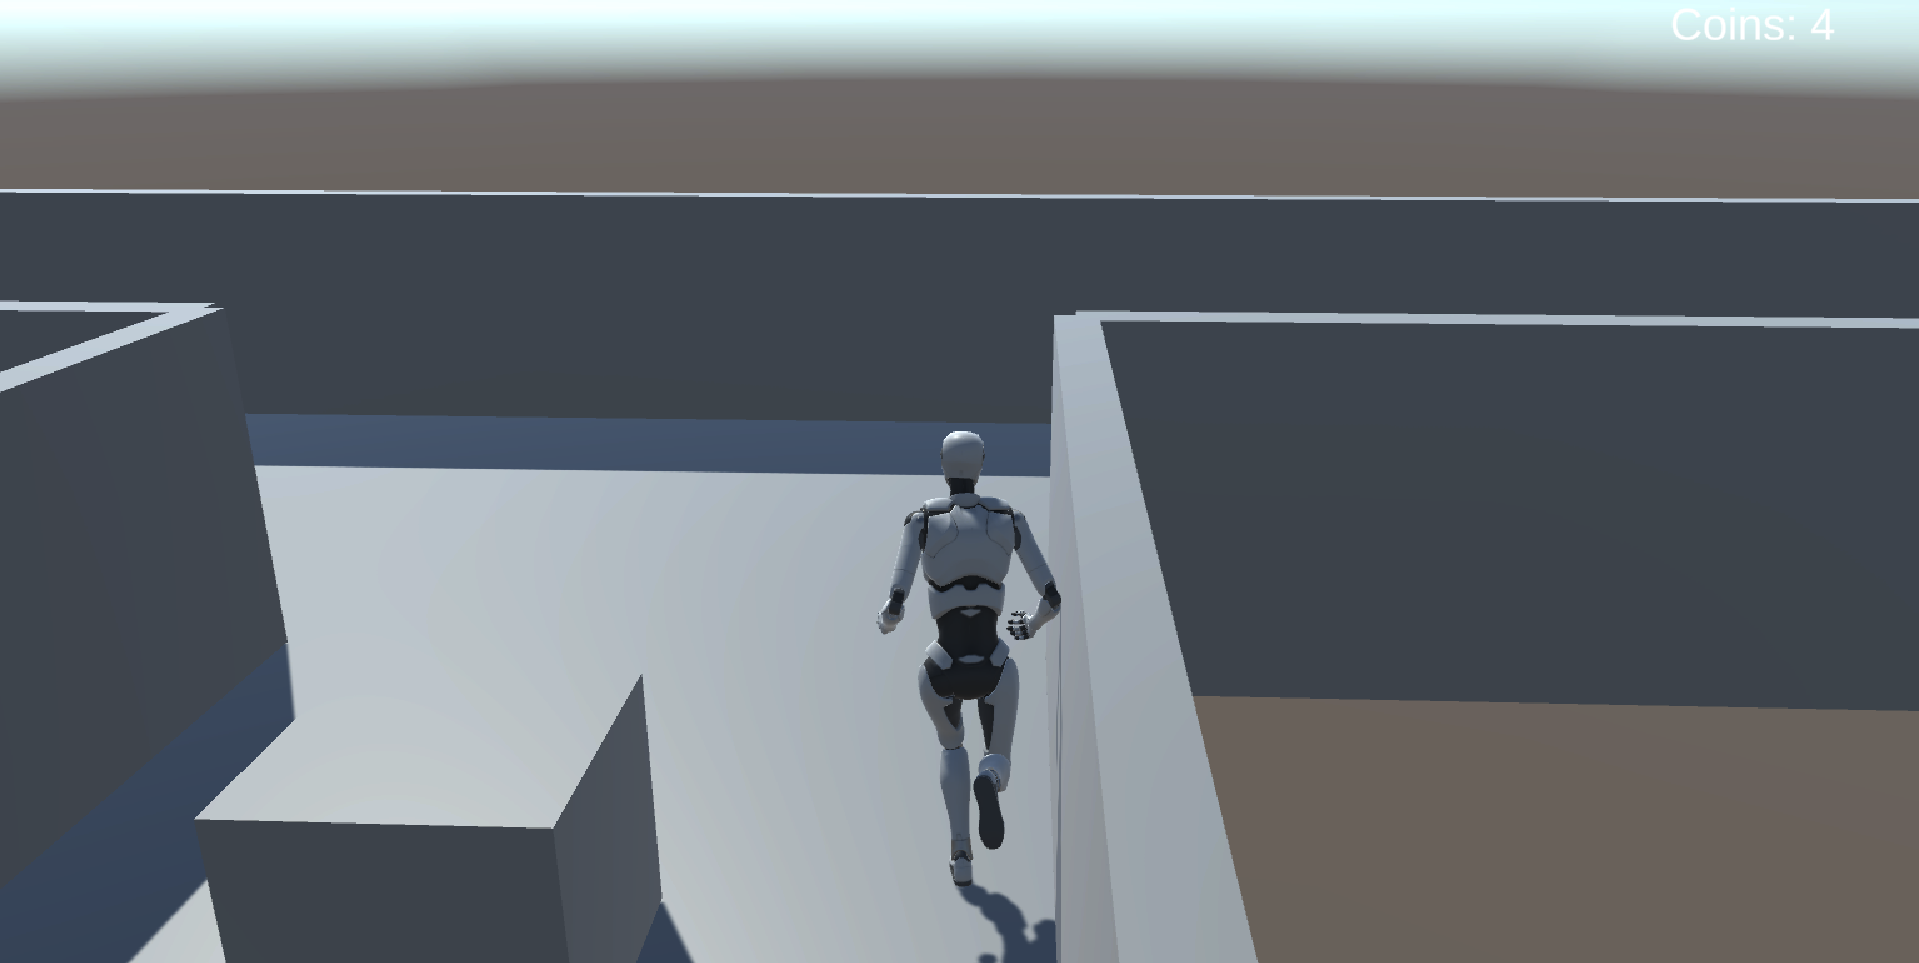
\includegraphics[width=0.8\textwidth]{Figures/Approach/infinite_runner}
    \caption{Infinite Runner Virtual Environment}
    \label{fig:infinite_runner}
\end{figure}

\begin{figure}[!htbp]
    \centering
    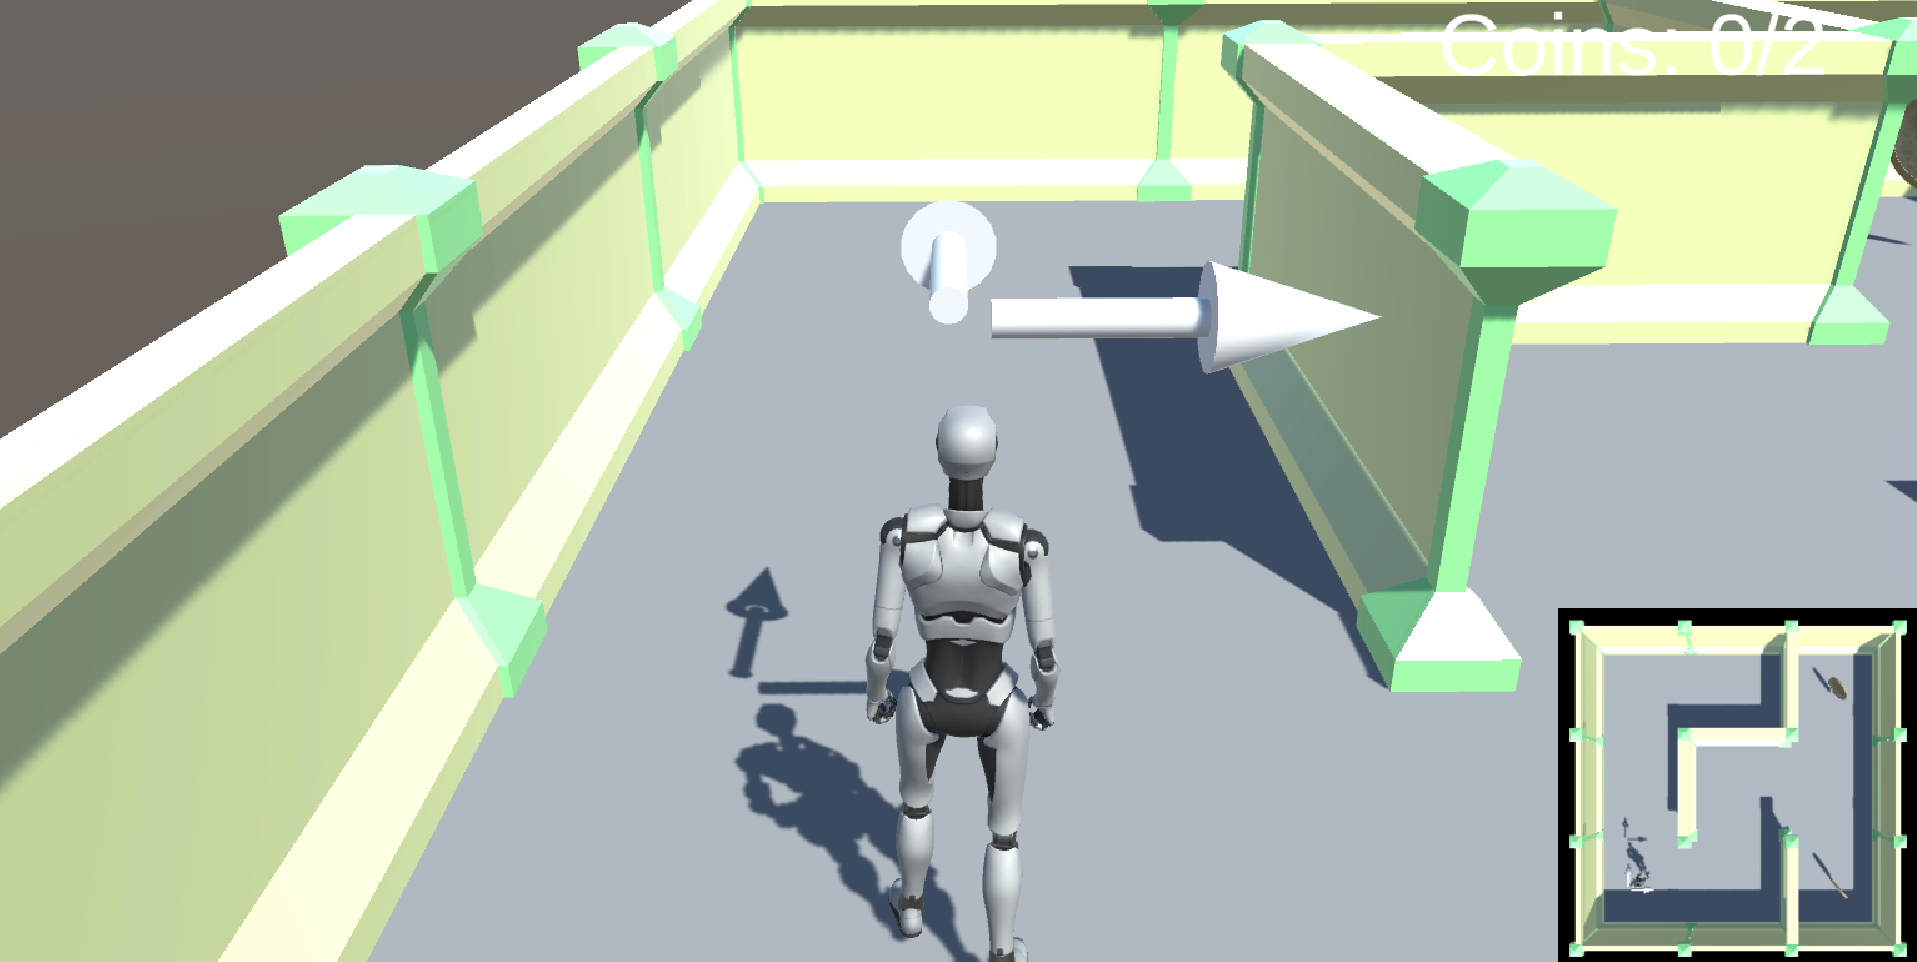
\includegraphics[width=0.8\textwidth]{Figures/Approach/maze}
    \caption{Maze Virtual Environment}
    \label{fig:maze}
\end{figure}

\section{The Framework}
To automate the process of data augmentation, model classification and game testing, we developed a framework that could be used to streamline the testing process.
The framework was designed to either generate new data or receive data from the EEG headset, classify the data, and then send the classification results to the virtual environment for testing.
The virtual environment would then provide feedback to the user by moving the virtual avatar based on the classification results.
The framework was developed using Python and PyTorch, and it was designed to be modular and extensible, so that new data augmentation techniques, classification models, and virtual environments could be easily added.
The framework was also designed to be easy to use, so that researchers and developers could quickly test new ideas and models without having to worry about the underlying implementation details.
The framework consists of three main components: the data augmentation module, the classification module, and the communication module.
The data augmentation module is responsible for generating new data samples using the data augmentation techniques, the classification module is responsible for classifying the data samples using the classification model, and the communication module is responsible for sending the classification results to other devices.
Currently, it is possible to specify the paths to the data augmentation and classification models, and the websocket address, in this way the framework can be easily adapted to different models and environments.

\begin{figure}[!htbp]
    \centering
    \begin{tikzpicture}[
        squarednode/.style={rectangle, draw=black, very thick, minimum size=5mm},
        ]
        \node[squarednode] (keyboard) {Keyboard Input};
        \node[squarednode] (data_augmentation) [below=of keyboard] {Data Augmentation};
        \node[squarednode] (classification) [right=of keyboard] {Classification};
        \node[squarednode] (websocket) [below=of classification] {Websocket};
        \node[squarednode] (virtual_environment) [right=of classification] {Virtual Environment};

        \draw[->] (keyboard) -- (data_augmentation);
        \draw[->] (data_augmentation) -- (classification);
        \draw[dashed, ->] (classification) -- (websocket);
        \draw[dashed, ->] (websocket) -- (virtual_environment);
    \end{tikzpicture}
\caption{High-level model of the framework}
\label{fig:framework}
\end{figure}
\todo{Explain the figure somewhere in the text}
